% Drawing 154/08-15 -- folder 154, batch 08, archive page 158 (PDF page 159).
% Transcription: croquis au crayon, sans texte suivi : un rectangle partagé par une horizontale, les deux moitiés marquées $\alpha$ et $\beta$, un cercle au crayon en surimpression ; un rectangle traversé d'un disque aplati et de courbes qui se tressent ; un ovale ; au-dessous, deux rectangles superposés traversés de courbes tressées, les coins et les bords marqués $v'$, $u'$, $a$, $b'$, $u$, $v$, $u'$, $a'$ (?), $a$, $u$, $v$, avec deux ellipses aux niveaux $a$ et $b'$ ; à côté, un disque aux courbes entrelacées. En bas à gauche, un dessin en couleur : deux bandes vert clair qui se rejoignent en un point noir de croisement, une droite rouge qui les longe et une droite rouge verticale, des hachures au crayon et de petites barres noires
% Kind: pencil sketches: rectangles with braided curves, an oval; coloured lines through a crossing. Method 2 (schematic redraw from the facsimile). Status: partial.
% Notes: Pencil sketches without running text, over a typed notice (not reproduced), read from the page view: a rectangle divided by a horizontal, the two halves marked alpha and beta, a pencil circle over it; a rectangle crossed by a flattened disk and by curves that braid; an oval; below, two stacked rectangles crossed by braided curves, sides marked (a, b', u ...; not reproduced), and a disk with braided strands; at the bottom, light green lines and a red line converging at a crossing with a red vertical. The curves are schematic.
% Coordinates: 1 unit = 1 mm = 1/100 of the crop width (bbox in page fractions: [0.152, 0.105, 0.474, 0.489]).
% Redrawn by Claude (claude-opus-5-5), issue #73, 2026-11-07; not checked by a human; not compiled (no TeX in the session).
% Rights: reproduces part of the work -- behind RENDER_TRANSCRIPTS, never published by itself.
\documentclass[tikz,border=3pt]{standalone}
\usepackage{amsmath,amssymb}
\usetikzlibrary{patterns,arrows.meta}
\tikzset{Or/.style={orange!90!black}, Ye/.style={yellow!80!orange}, Lg/.style={green!60!black!70}, Dg/.style={green!45!black}, Br/.style={brown!80!black}, Rd/.style={red!85!black}, Bl/.style={blue!70!black}, Gy/.style={black!40}, pencil/.style={black!45}, struck/.style={black!35}, mark/.style={circle,draw,inner sep=1.3pt}, pt/.style={circle,fill,inner sep=0.9pt}, opt/.style={circle,draw,fill=white,inner sep=1.1pt}}
\begin{document}
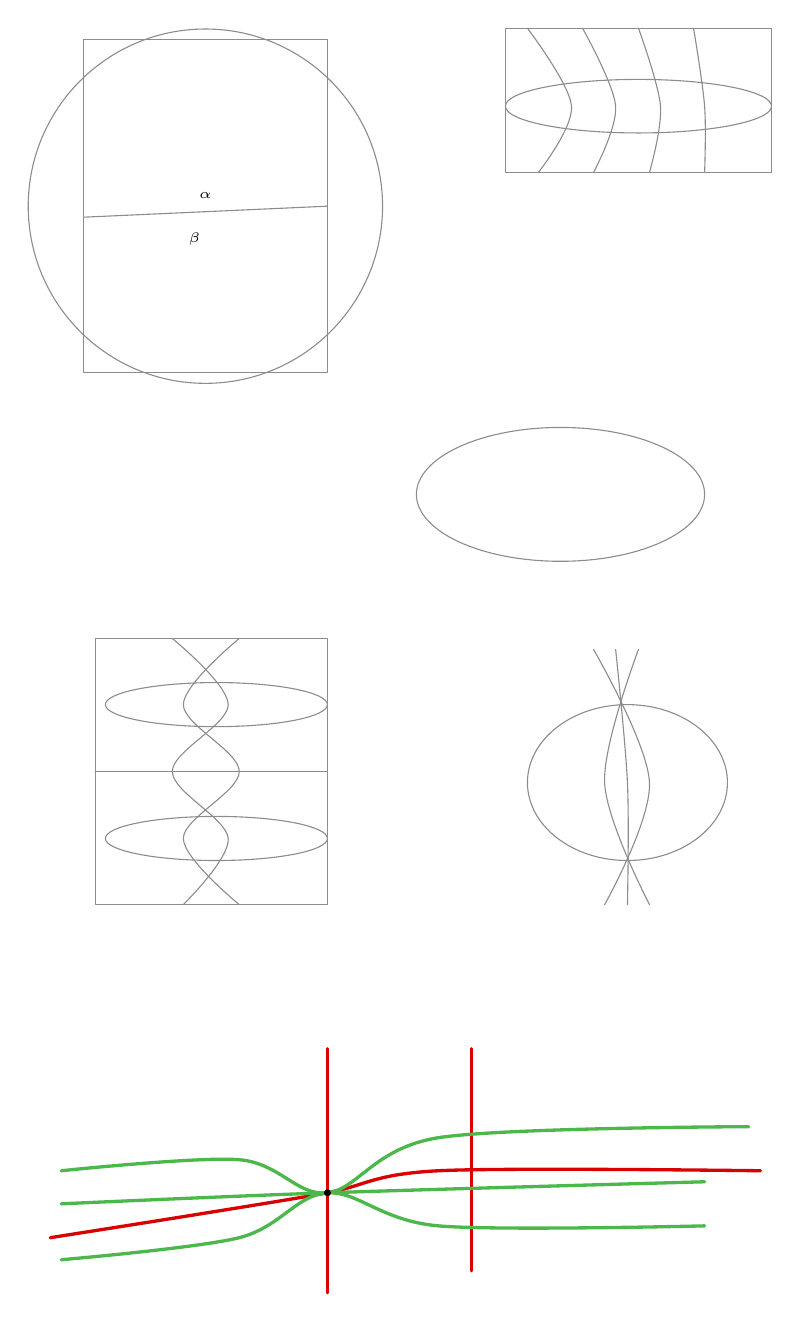
\begin{tikzpicture}[x=1mm,y=1mm,line cap=round,line join=round,font=\scriptsize]
\draw[pencil] (7,-7) -- (38,-7) -- (38,-49.3) -- (7,-49.3) -- cycle;
\draw[pencil] (7,-29.6) -- (38,-28.2);
\node[inner sep=1pt] at (22.5,-26.8) {\tiny $\alpha$};
\node[inner sep=1pt] at (21.1,-32.4) {\tiny $\beta$};
\draw[pencil] (22.5,-28.2) circle[radius=22.5];
\draw[pencil] (60.6,-5.6) -- (94.4,-5.6) -- (94.4,-23.9) -- (60.6,-23.9) -- cycle;
\draw[pencil] (77.5,-15.5) ellipse[x radius=16.9, y radius=3.4];
\draw[pencil] plot[smooth, tension=0.55] coordinates {(63.4,-5.6) (69,-15.5) (64.8,-23.9)};
\draw[pencil] plot[smooth, tension=0.55] coordinates {(70.4,-5.6) (74.6,-15.5) (71.8,-23.9)};
\draw[pencil] plot[smooth, tension=0.55] coordinates {(77.5,-5.6) (80.3,-15.5) (78.9,-23.9)};
\draw[pencil] plot[smooth, tension=0.55] coordinates {(84.5,-5.6) (85.9,-15.5) (85.9,-23.9)};
\draw[pencil] (67.6,-64.8) ellipse[x radius=18.3, y radius=8.5];
\draw[pencil] (8.5,-83.1) -- (38,-83.1) -- (38,-116.9) -- (8.5,-116.9) -- cycle;
\draw[pencil] (8.5,-100) -- (38,-100);
\draw[pencil] plot[smooth, tension=0.55] coordinates {(18.3,-83.1) (25.4,-91.5) (18.3,-100) (25.4,-108.5) (19.7,-116.9)};
\draw[pencil] plot[smooth, tension=0.55] coordinates {(26.8,-83.1) (19.7,-91.5) (26.8,-100) (19.7,-108.5) (26.8,-116.9)};
\draw[pencil] (23.9,-91.5) ellipse[x radius=14.1, y radius=2.8];
\draw[pencil] (23.9,-108.5) ellipse[x radius=14.1, y radius=2.8];
\draw[pencil] (76.1,-101.4) ellipse[x radius=12.7, y radius=9.9];
\draw[pencil] plot[smooth, tension=0.55] coordinates {(71.8,-84.5) (78.9,-101.4) (73.2,-116.9)};
\draw[pencil] plot[smooth, tension=0.55] coordinates {(74.6,-84.5) (76.1,-101.4) (76.1,-116.9)};
\draw[pencil] plot[smooth, tension=0.55] coordinates {(77.5,-84.5) (73.2,-101.4) (78.9,-116.9)};
\draw[Rd,very thick] plot[smooth, tension=0.55] coordinates {(2.8,-159.2) (21.1,-156.3) (38,-153.5) (52.1,-150.7) (93,-150.7)};
\draw[Rd,very thick] (38,-135.2) -- (38,-166.2);
\draw[Rd,very thick] (56.3,-135.2) -- (56.3,-163.4);
\draw[Lg,very thick] plot[smooth, tension=0.55] coordinates {(4.2,-150.7) (26.8,-149.3) (38,-153.5) (52.1,-146.5) (91.5,-145.1)};
\draw[Lg,very thick] plot[smooth, tension=0.55] coordinates {(4.2,-162) (26.8,-159.2) (38,-153.5) (52.1,-157.7) (85.9,-157.7)};
\draw[Lg,very thick] plot[smooth, tension=0.55] coordinates {(4.2,-154.9) (38,-153.5) (85.9,-152.1)};
\node[pt] at (38,-153.5) {};
\end{tikzpicture}
\end{document}
